In this report, the main project choices and the results for structural ensemble PED00020 of measles virus nucleoprotein (for its five deposited ensembles) are reported.

\section{Task 1}\label{sec:task1}
\graphicspath{ {./figures/} }
The goal of the first task is to implement a tool to identify conformational relationships thanks to models structural features within an ensemble. The input is a set of files, each containing the PDB structure of one ensemble, which will be analyzed independently.

\subsection{Single conformation features}

For each conformation, the following structural features are extracted and subsequently saved:
\begin{itemize}
\item[-] \emph{Radius of gyration} is computed from the coordinates of each atom and their barycenter.
\item[-] \emph{Relative accessible surface area} (ASA) is computed for each residue thanks to DSSP\footnote{\textbf{DSSP}: the values obtained for the conformations within an ensemble are equal. It may happen that the DSSP does not return the ASA value for some residues: for this limitation, a check on the array dimension and, if needed, a zero-padding are performed. }.
\item[-] \emph{Secondary structure} (SS) is determined for each residue thanks to the Ramachandran regions\footnote{\textbf{SS}: for the first and last residue, for which the value is not computable, `-' is inserted.} associated to Phi and Psi angles. For an easiest subsequent analysis, each value is converted into an integer as reported in table \ref{tab:ss}.
\item[-] \emph{Distance matrix} contains the pairwise distances between each pair of residues. For an easiest analysis, since it is symmetric, only the linearized version of its upper triangular sub-matrix is considered.
\end{itemize}

\begin{table}[H]
\begin{center}
\begin{tabular}{lc}
% FIRST ROW
\textbf{Secondary Structure} & \textbf{Int}\\
\hline
- & 0\\
\hline
Beta-sheet & 1\\
\hline
Polyproline I-II & 2\\
\hline
Alpha-helix & 3\\
\hline
Left-handed Helix & 4\\
\end{tabular}
\end{center}
\caption{Conversion for Secondary Structure values}~\label{tab:ss}
\end{table}


\subsection{Representative conformations}
In order to extract the representative conformations, the models are clustered due to \emph{K-Medoids} approach and a customized metric function, selecting the optimal number of clusters thanks to Silhouette score.
\emph{K-Medoids} has been chosen since centroids are selected between the input set points, without generating unseen conformations.

\medskip
The implemented metric\footnote{\textbf{Metric}: take in input feature vectors of two conformations and compute their distance as sum of partial features distances.} is tailored for each feature set, in order to measure the dissimilarity between models. The distance metrics have been chosen according to the meaning and the behavior of single features. %Scrivere che consideriamo le seguenti cose:
\begin{itemize}
\item[-] Absolute difference between radius of gyration to understand its variation.
\item[-] Euclidean distance of ASA vectors.
\item[-] Normalized Hamming distance between SS vectors using a scoring matrix accordingly to their definition and properties. The scoring matrix is reported in table \ref{tab:score}.

\begin{table}[H]
\begin{center}
\begin{tabular}{c|ccccc}
% FIRST ROW
& 0 & 1 & 2 & 3 & 4 \\
\hline
0 & 0 & 1 & 1 & 1 & 1\\
1 & 1 & 0 & 1 & 1 & 1\\
2 & 1 & 1 & 0 & 1 & 1\\
3 & 1 & 1 & 1 & 0 & 0.5\\
4 & 1 & 1 & 1 & 0.5 & 0\\
\end{tabular}
\end{center}
\caption{Scoring matrix Secondary Structure values}~\label{tab:score}
\end{table}

\item[-] The cosine distance between distance matrix. 
\end{itemize}

In table \ref{tab:silhouette} we report both the optimal number of clusters and the corresponding silhouette scores obtained with the described clustering procedure. 
Once the representative conformations are extracted as centroids, the software plots a weighted graph, where each node is a representative model and the edge length is proportional to the distance between each pair of conformations according to the metric function; the distance is reported also as correspondent edge label.

\begin{table}[H]
\begin{center}
\begin{tabular}{ccc}
% FIRST ROW
\textbf{Ensemble} & \textbf{Cluster} & \textbf{Silhouette}\\
\hline
001 & 4 & 0.538269\\
\hline
002 & 3 & 0.511878\\
\hline
003 & 4 & 0.499020\\
\hline
004 & 3 & 0.521289\\
\hline
005 & 3 & 0.545507\\
\end{tabular}
\end{center}
\caption{Silhouette values obtained during clustering}~\label{tab:silhouette}
\end{table}

\begin{figure}[H]
    \centering
	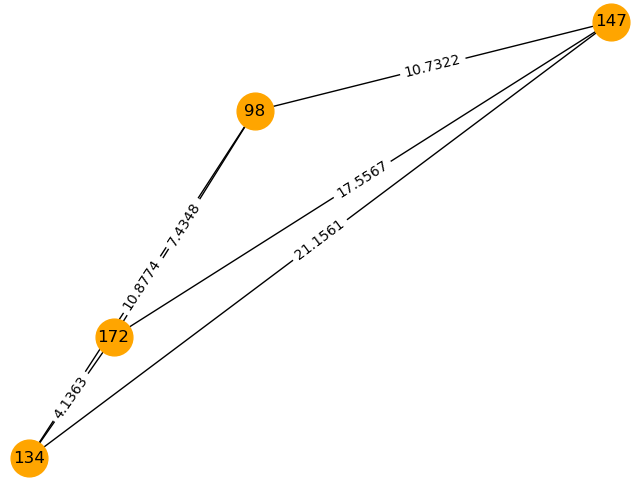
\includegraphics[width=\textwidth]{PED00020e001_graph.png}
	\caption{Graph of ensemble 001.}
	\label{model001}
\end{figure}

\begin{figure}[H]
    \centering
		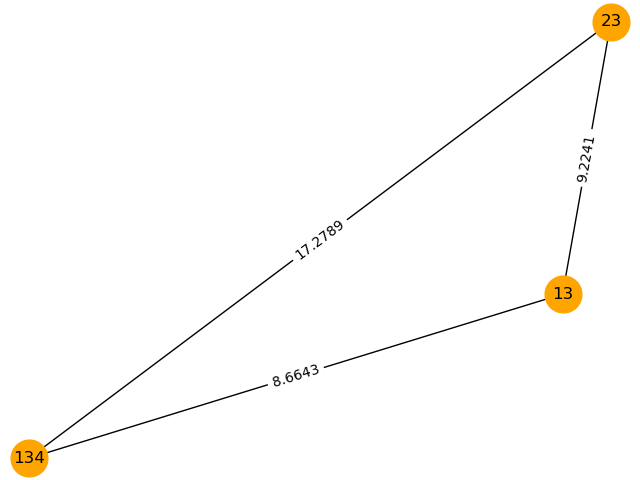
\includegraphics[width=\textwidth]{PED00020e002_graph.png}
		\caption{Graph of ensemble 002.}
		\label{model002}
\end{figure}

\begin{figure}[H]
    \centering
		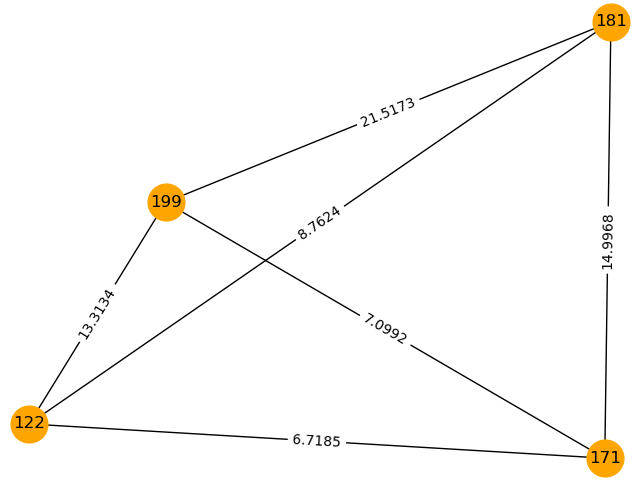
\includegraphics[width=\textwidth]{PED00020e003_graph.png}
		\caption{Graph of ensemble 003.}
		\label{model003}
\end{figure}

\begin{figure}[H]
    \centering
		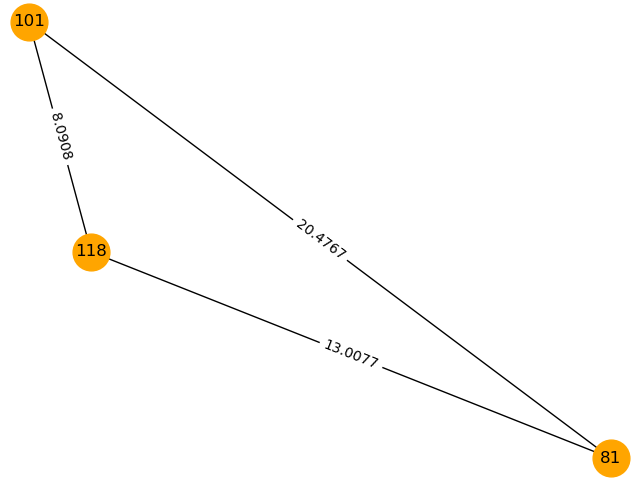
\includegraphics[width=\textwidth]{PED00020e004_graph.png}
		\caption{Graph of ensemble 004.}
		\label{model004}
\end{figure}

\begin{figure}[H]
    \centering
		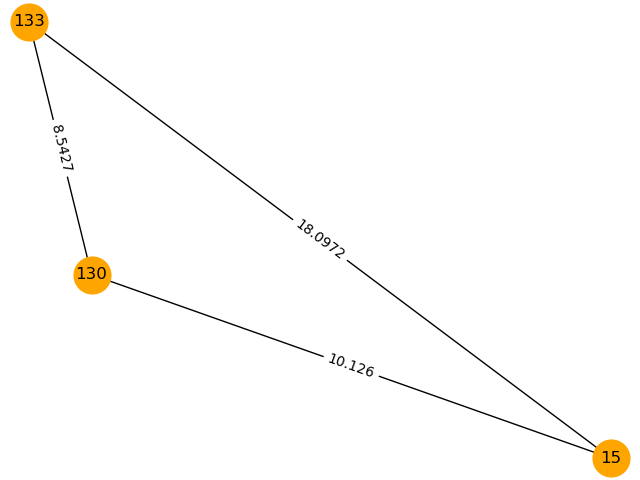
\includegraphics[width=\textwidth]{PED00020e005_graph.png}
		\caption{Graph of ensemble 005.}
		\label{model005}
\end{figure}


In figures \ref{model001}, \ref{model002}, \ref{model003}, \ref{model004} and \ref{model005} the obtained graphs are reported. By running the script several times, a high results variability can be observed.
This is probably caused by the proximity of the points (represented in the features space) and the random initialization of clustering. The centroids are usually different but found in the same cardinality.



\subsection{Pymol image}
For each ensemble, we decide to generate one Pymol image to visualize the 3D structure of one representative conformation and the variability of each residue in terms of features through the changing of the color. 

As a matter of fact, the generation of an image representating the conformations superimposition would give a too messy result and would not reporting important information. 
Another limitation has been the computing time needed for the features comparison: indeed, considering the residue variability over all the models, the time needed only for the Pymol image generation is about one hour. For this reason, we have decided to take into consideration only the representative conformations extracted by clustering step for the subsequent analysis since each of these conformations is a good approximation of its cluster.

\medskip
The residue variability is calculated using a metric built by us that considers the neighbors of the residue under analysis thanks to a window of size 9 on the left and on the right of the current position and extract the features vectors of those residues for each considered conformation. 
The metric then calculates the variability as the sum of the following partial distances:
\begin{itemize}
\item[-] Standard deviation of ASA values available for each residue is calculated and the mean of them is subsequently calculated to have an average value.
\item[-] Normalized distance between SS vectors pairs is calculated using the scoring matrix reported in table \ref{tab:ss}.
\item[-] For each pair of analyzed conformation, the cosine dissimilarity between distance vectors (rows/columns of distance matrix) of corresponding residues are summed.
\end{itemize}
Note that the radius of gyration is not used since it is not residue-dependent.

\begin{figure}[H]
    \centering
		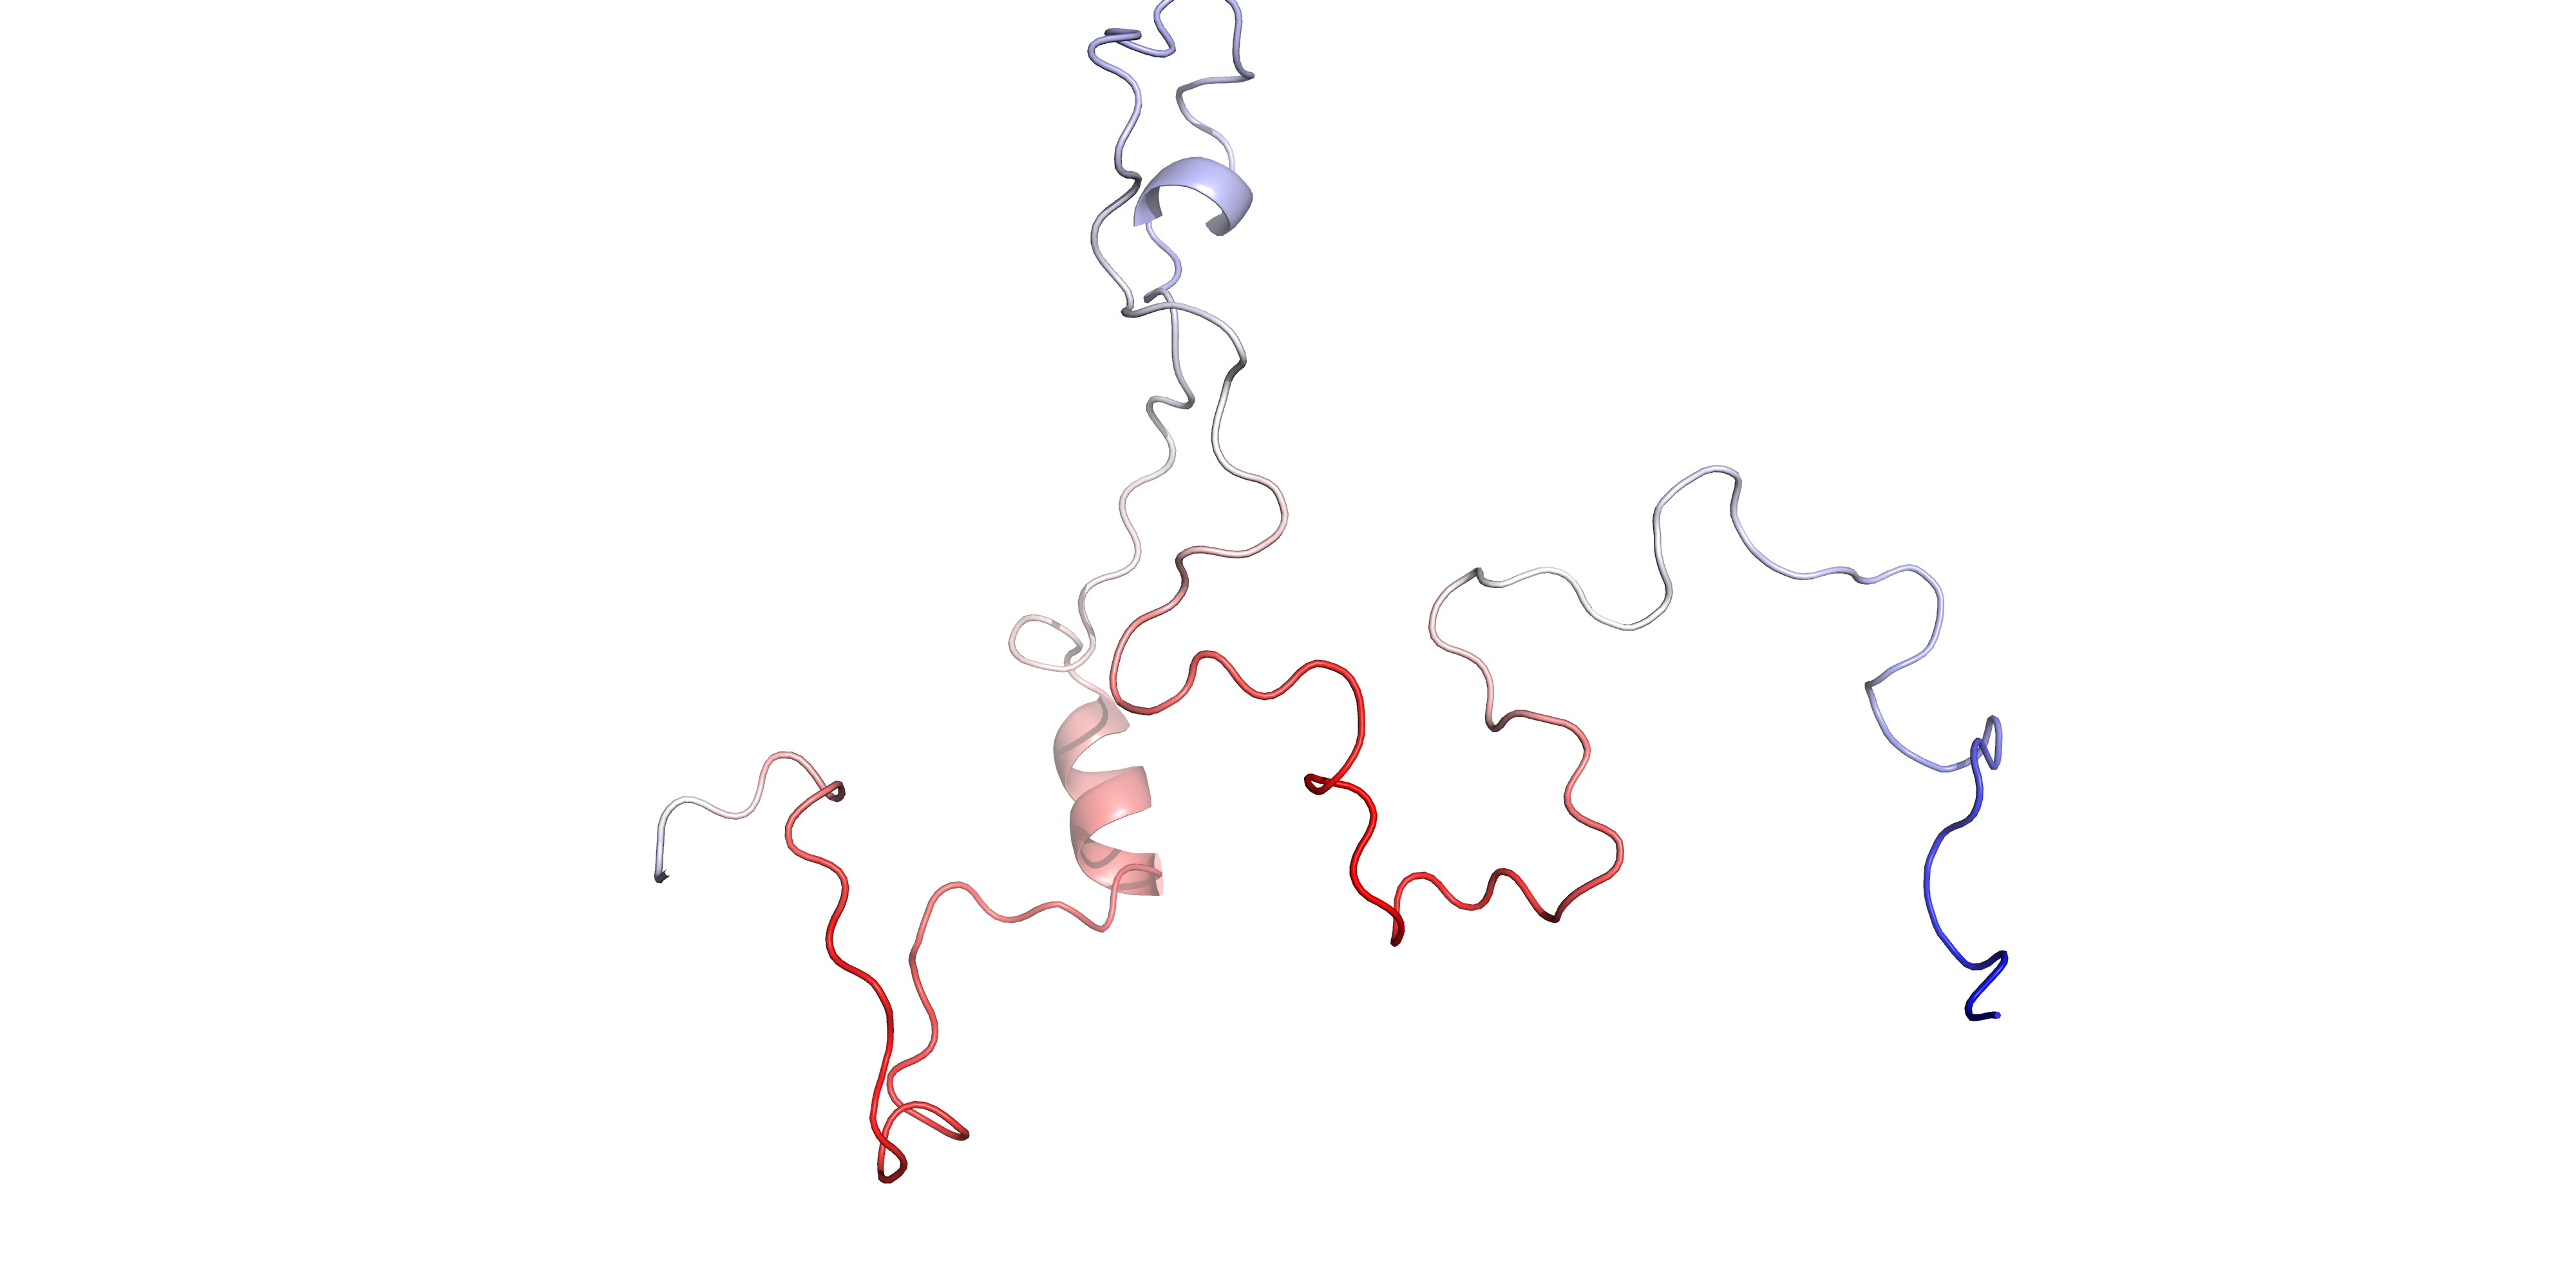
\includegraphics[width=\textwidth]{PED00020e001_pymol.png}
		\caption{Pymol image of ensemble 001 (model 098).}
		\label{model001p}
\end{figure}

\begin{figure}[H]
    \centering
		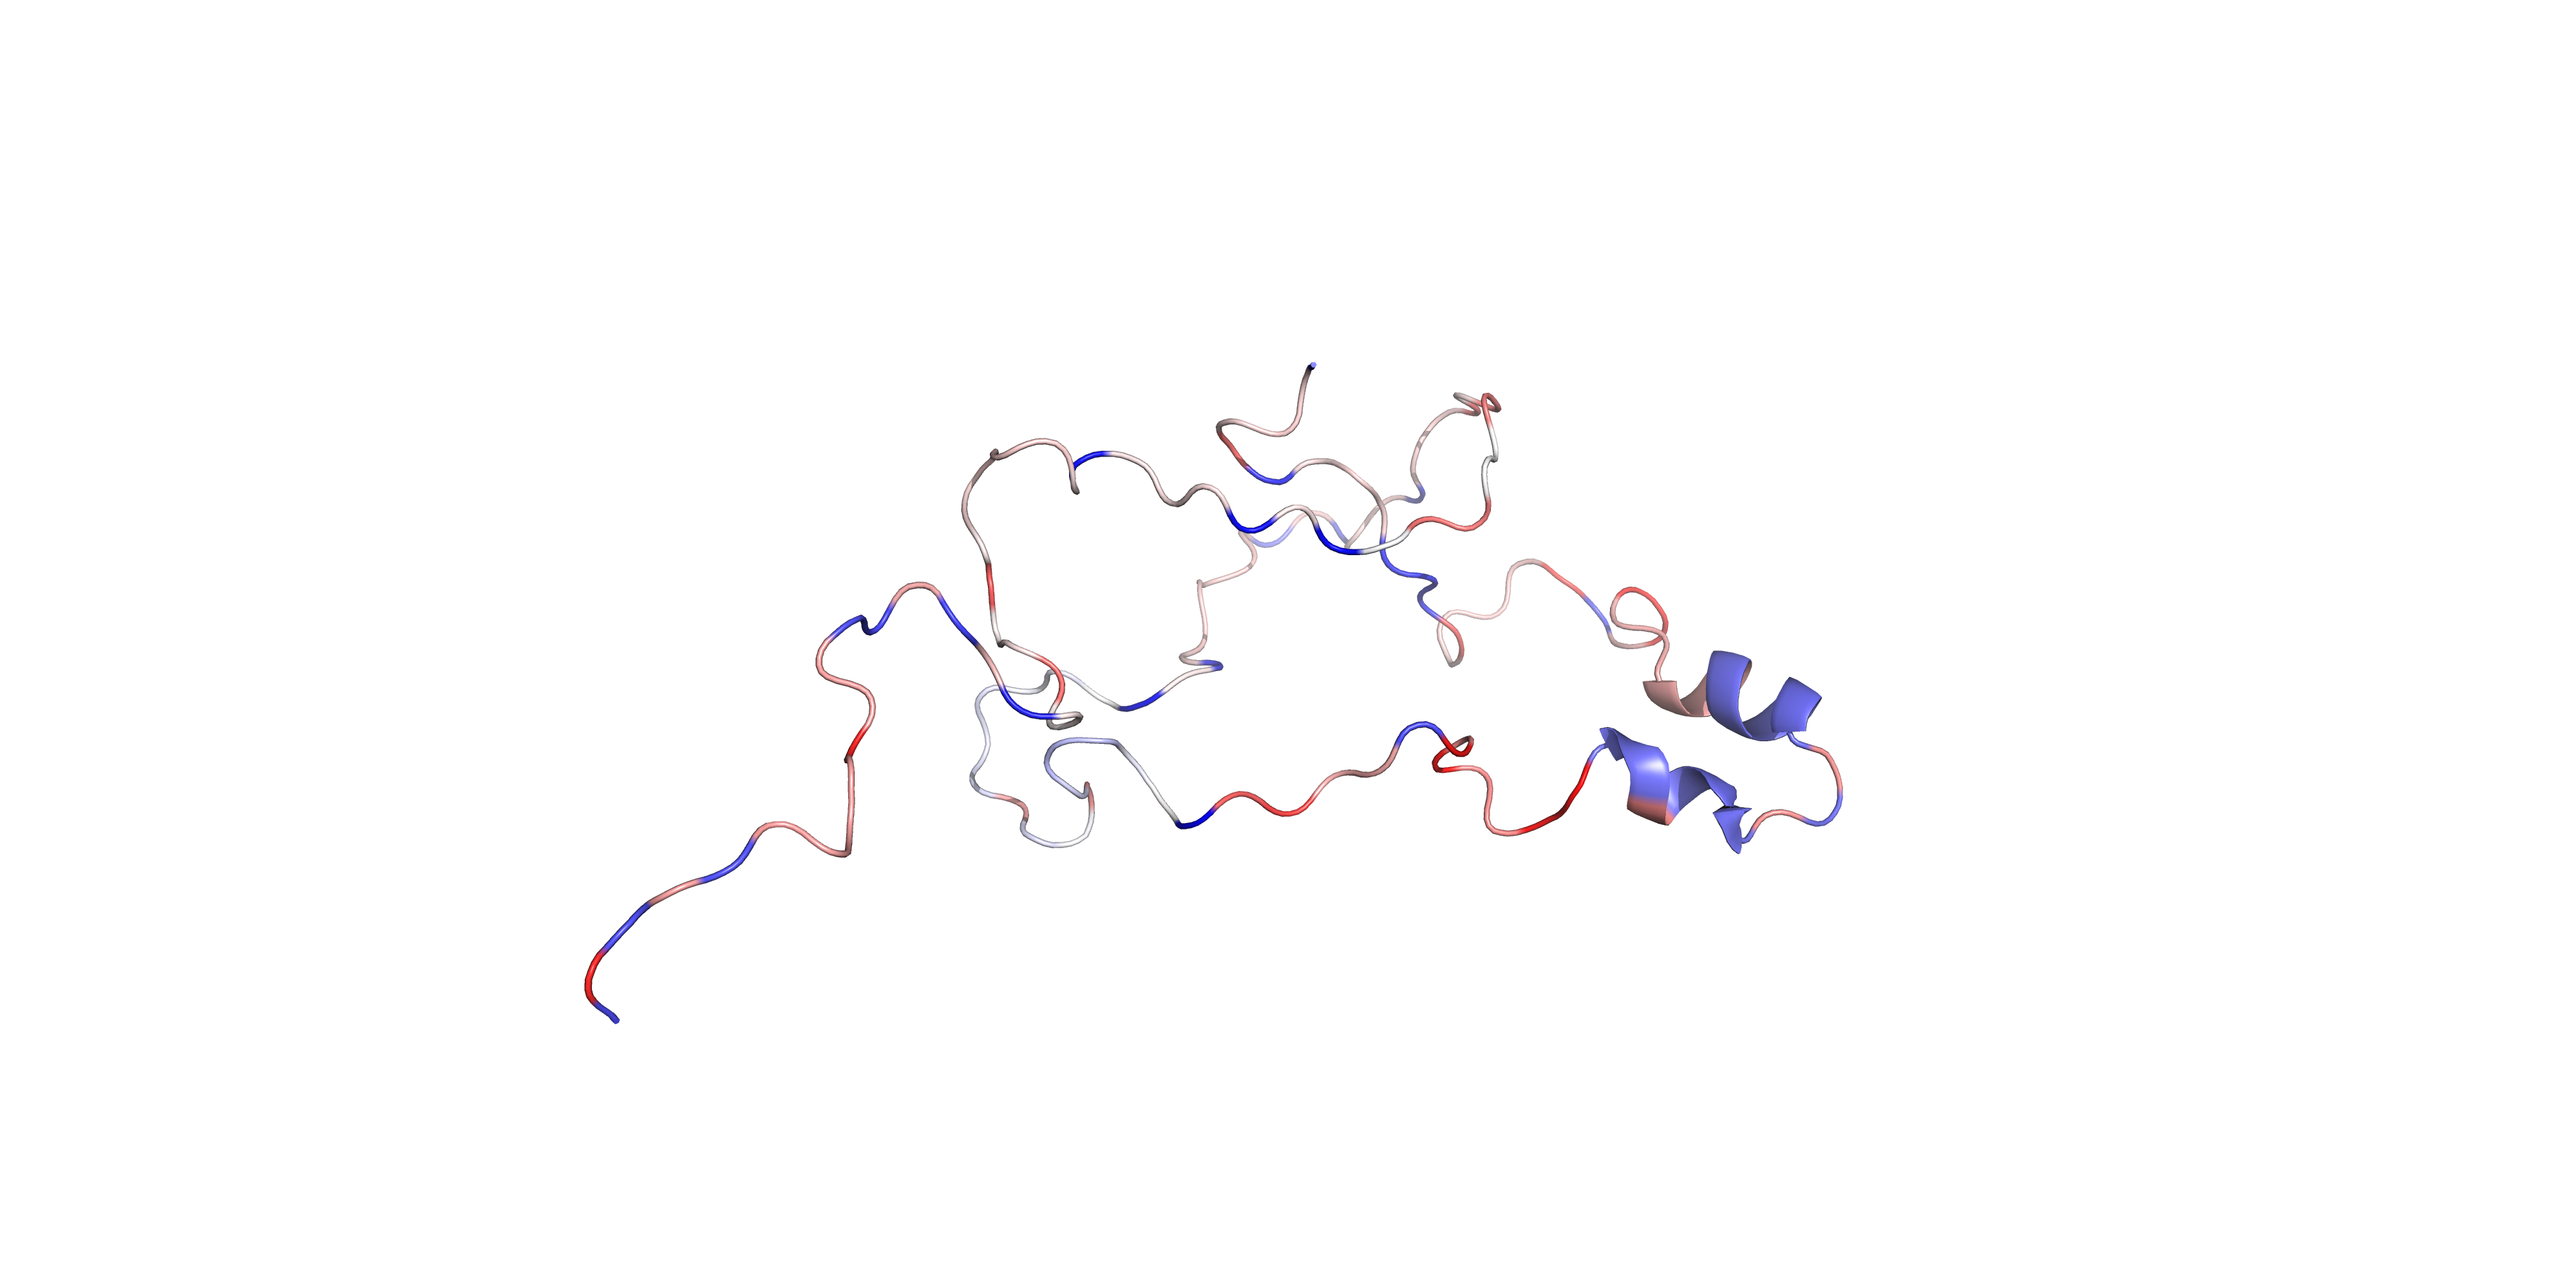
\includegraphics[width=\textwidth]{PED00020e002_pymol.png}
		\caption{Pymol image of ensemble 002 (model 023).}
		\label{model002p}
\end{figure}

\begin{figure}[H]
    \centering
		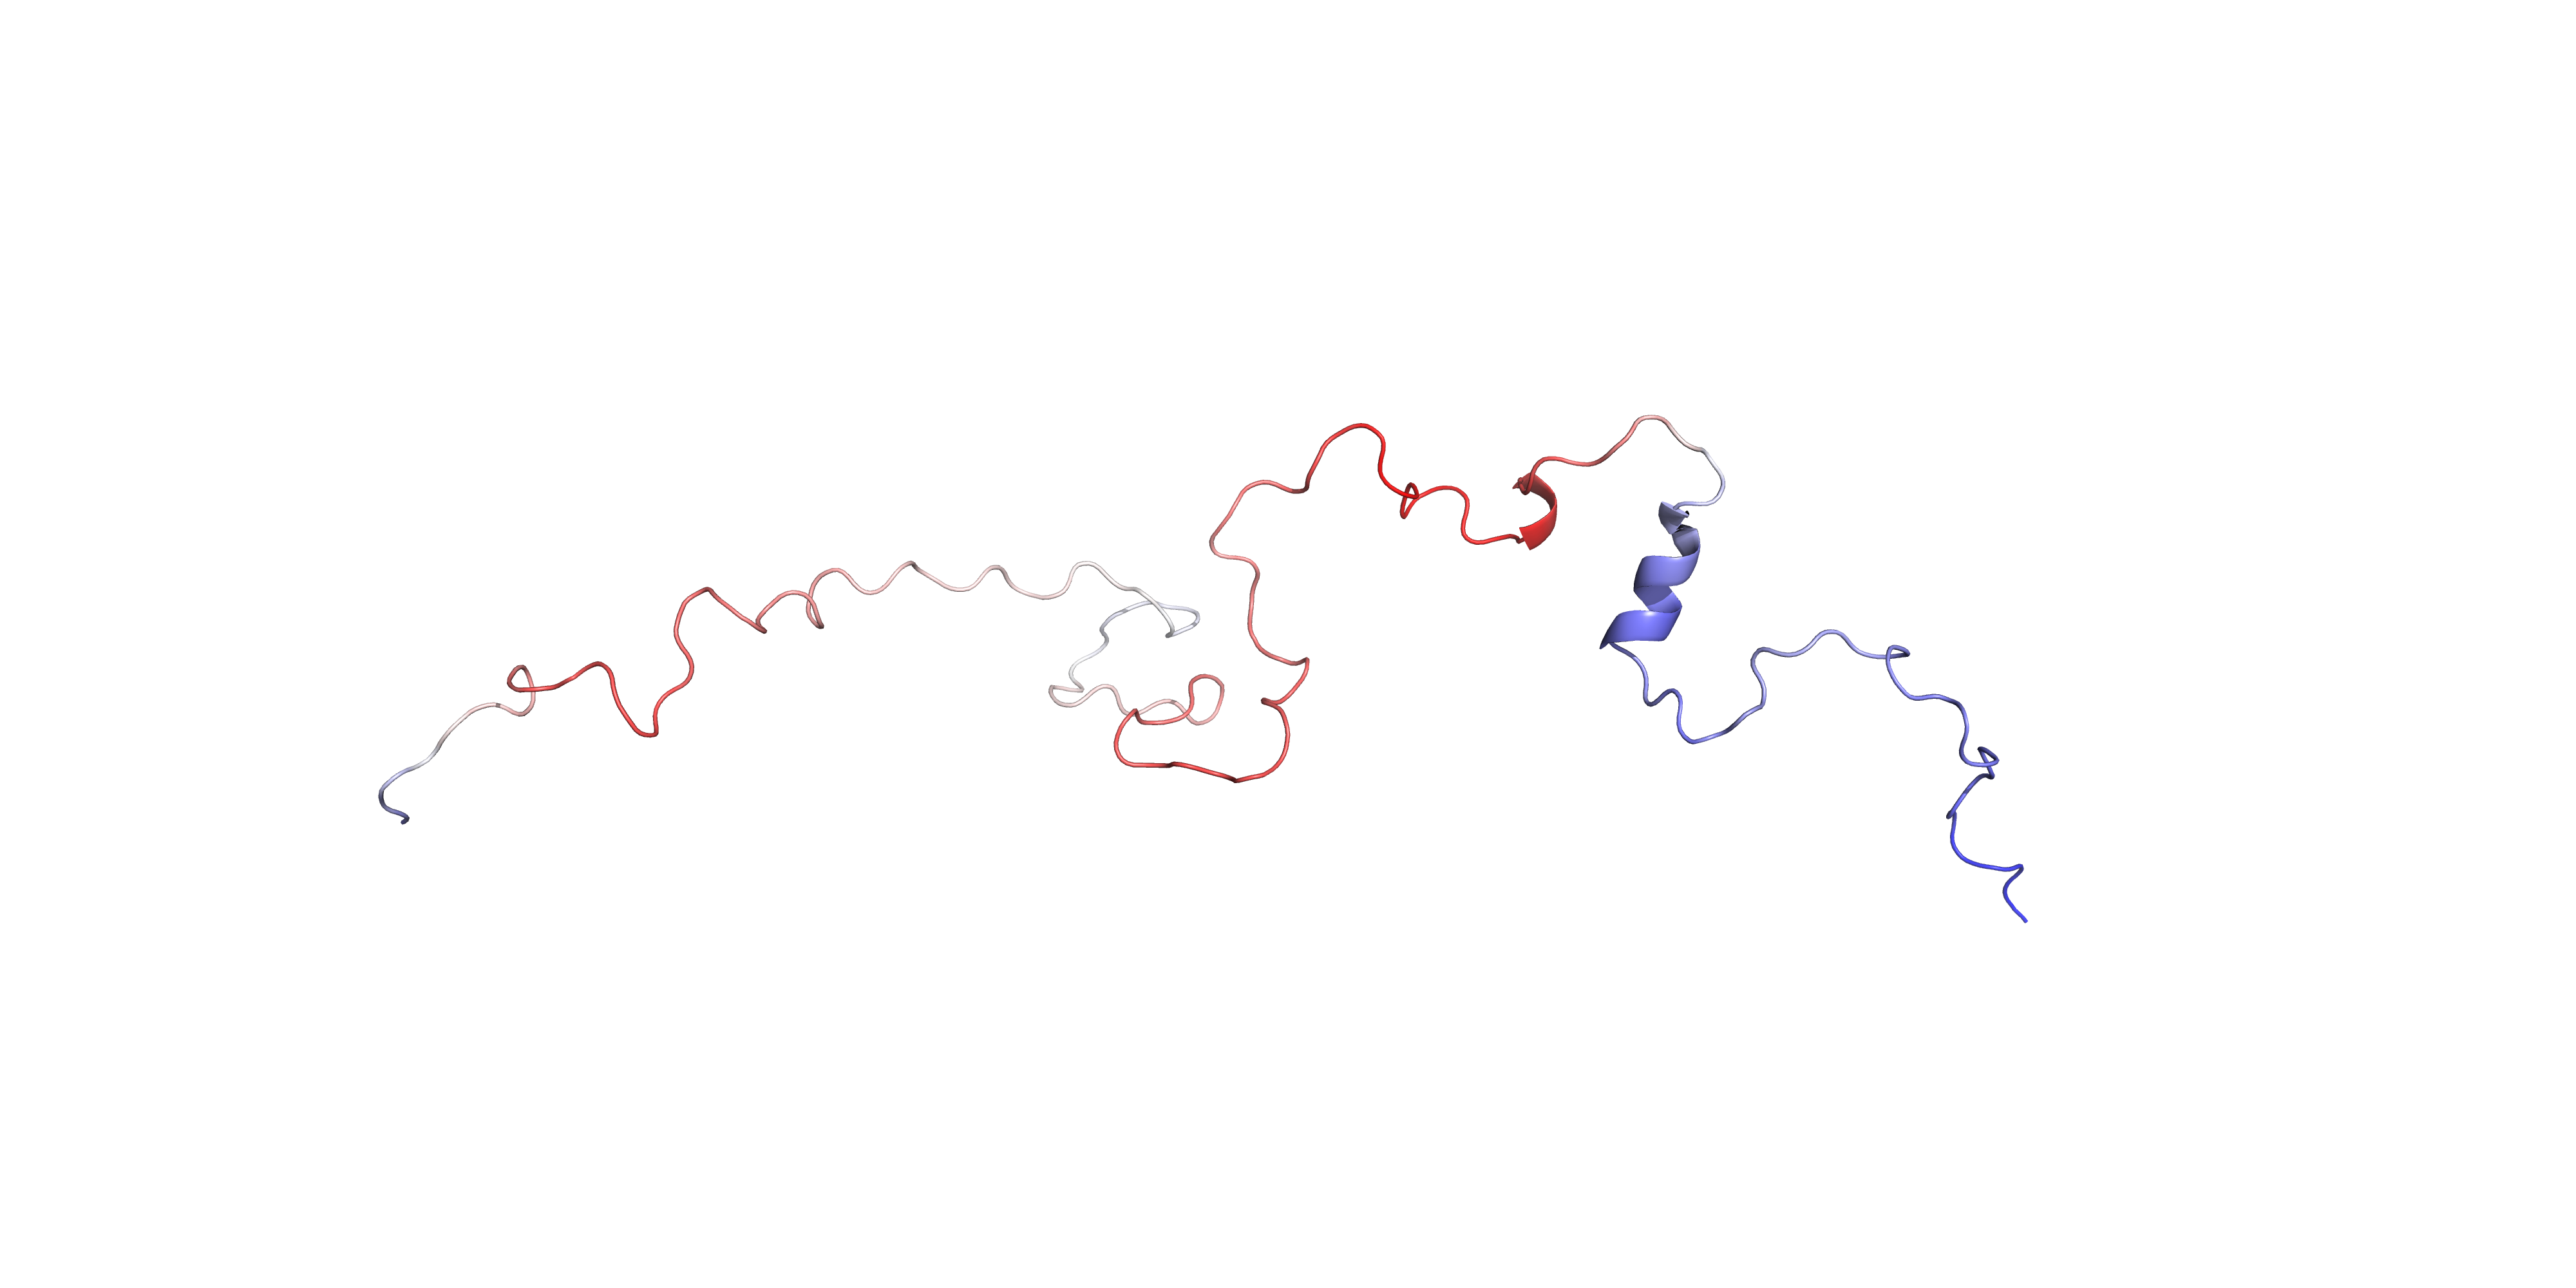
\includegraphics[width=\textwidth]{PED00020e003_pymol.png}
		\caption{Pymol image of ensemble 003 (model 122).}
		\label{model003p}
\end{figure}

\begin{figure}[H]
    \centering
		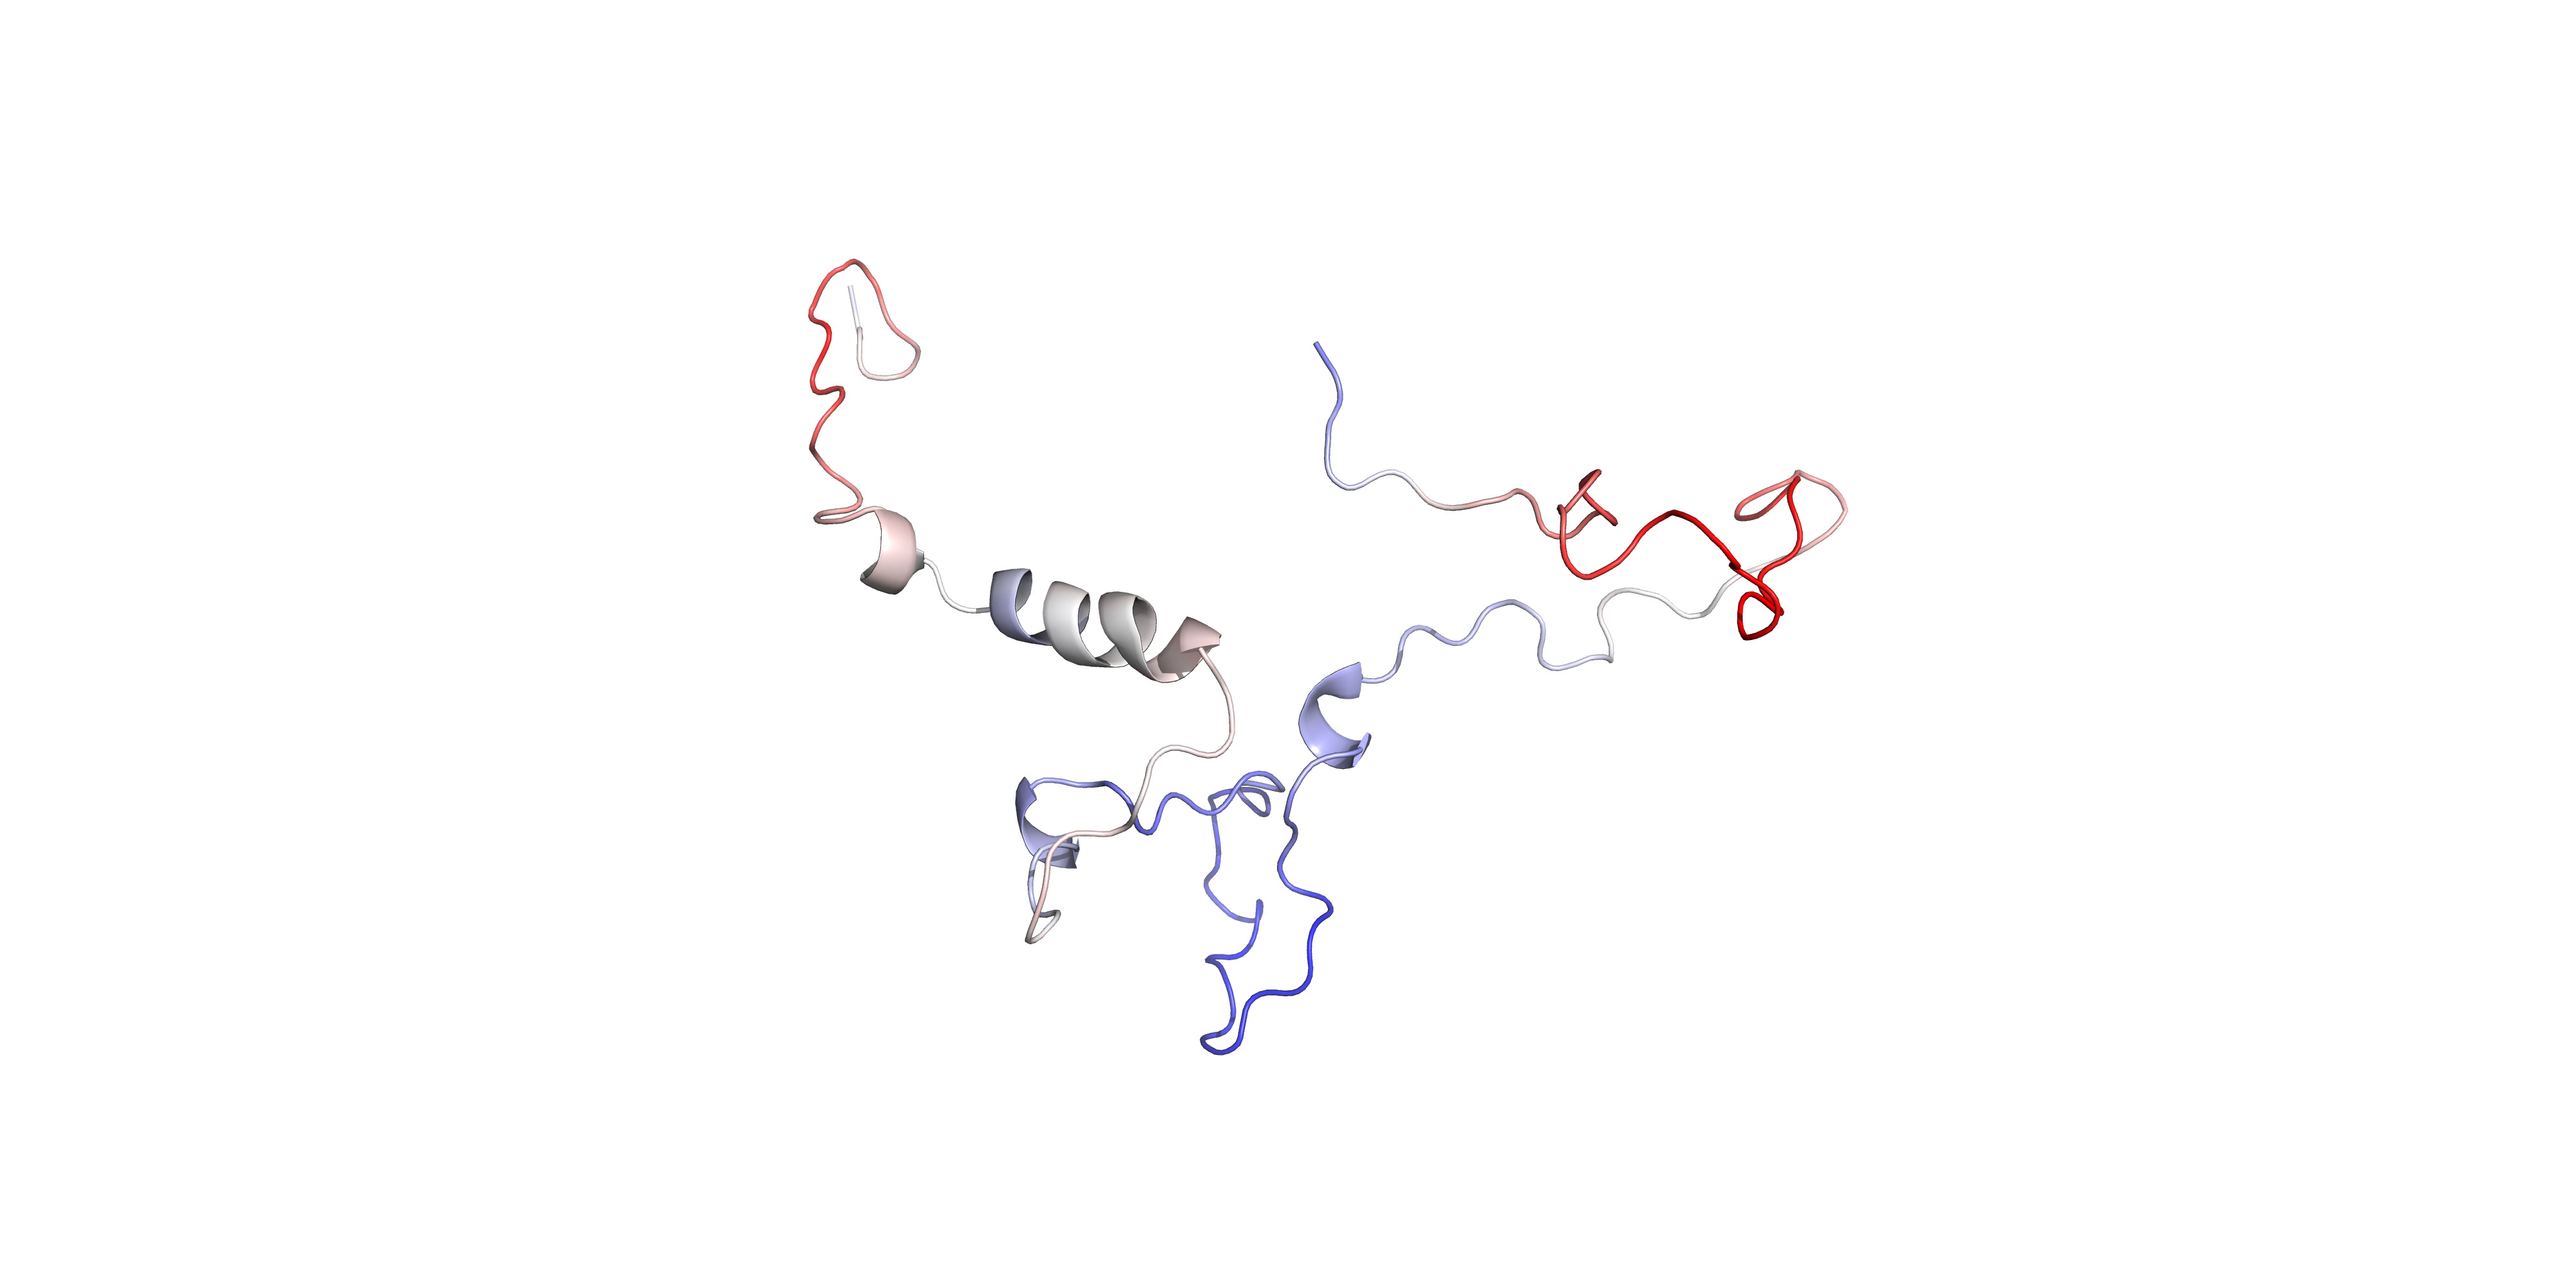
\includegraphics[width=\textwidth]{PED00020e004_pymol.png}
		\caption{Pymol image of ensemble 004 (model 118).}
		\label{model004p}
\end{figure}

\begin{figure}[H]
    \centering
		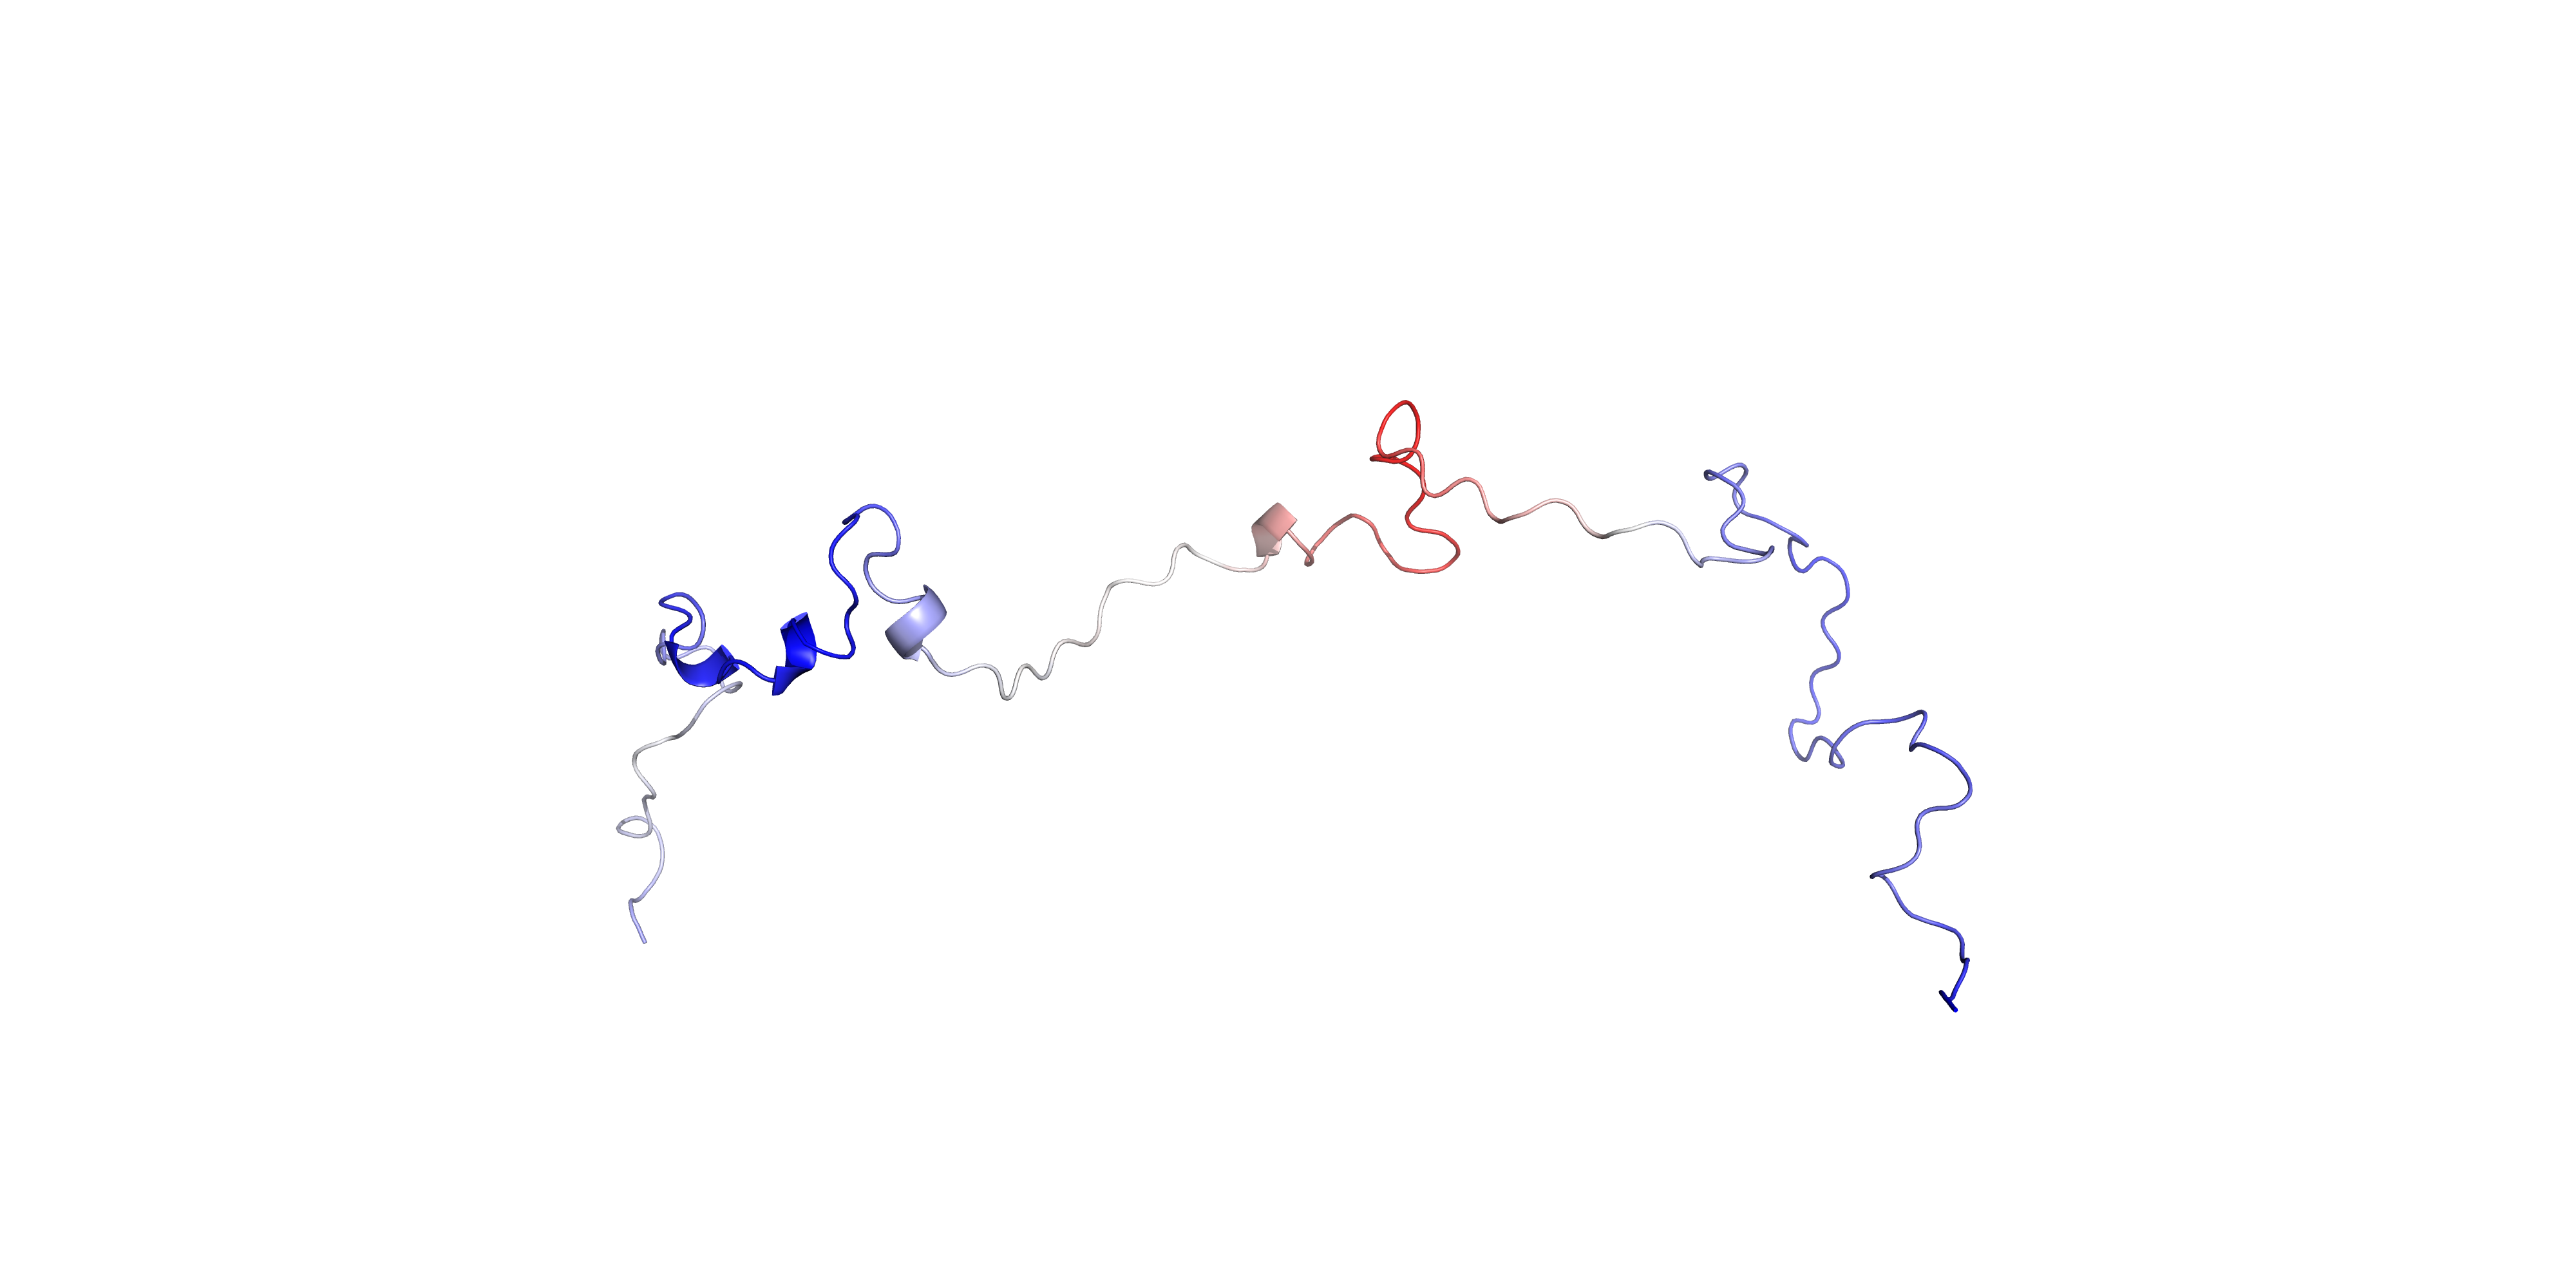
\includegraphics[width=\textwidth]{PED00020e005_pymol.png}
		\caption{Pymol image of ensemble 005 (model 133).}
		\label{model005p}
\end{figure}


\medskip
\medskip
In Pymol image, the color variability corrispond to red for the residues in the structure with high variability with respect to the features considered, while blue identifies the most stable areas. Also intermediate scenarios are displayed with color shades of red or blue.  

\medskip
Looking at figures \ref{model001p}, \ref{model002p}, \ref{model003p}, \ref{model004p} and \ref{model005p}, it is possible to see that the visualized structures are very disordered. Due to the entropic high cost of folding, the well-defined structures (e.g. alpha-helix) are not many. %da aggiungere basato sui nuovi grafici
